\documentclass[11pt]{article}

\usepackage[margin=1in]{geometry}
\usepackage{amsmath,amssymb}
\usepackage{booktabs}
\usepackage{tabularx}
\usepackage{array}
\usepackage{enumitem}
\usepackage{xcolor}
\usepackage{xurl}
\usepackage{hyperref}
\usepackage{fancyhdr}
\usepackage{microtype}
\usepackage{graphicx}
\usepackage{float}

\hypersetup{
    colorlinks=true,
    linkcolor=blue,
    urlcolor=blue,
    citecolor=blue,
    pdftitle={UAV Launch System Actuator Component Selection}
}

\newcommand{\ValuesDoc}{\texttt{actuator\_force\_requirements.tex} / \texttt{actuatorValues.py}}
\newcommand{\OptionsDoc}{\texttt{actuator\_part\_comparison.tex}}

\newcolumntype{Y}{>{\raggedright\arraybackslash}X}
\setlength{\parindent}{0pt}
\setlength{\parskip}{0.55em}
\renewcommand{\arraystretch}{1.18}

\pagestyle{fancy}
\fancyhf{}
\lhead{UAV Launch System}
\rhead{Actuator Component Selection}
\cfoot{\thepage}
\setlength{\headheight}{14pt}

\begin{document}
\pagenumbering{roman}

\begin{titlepage}
    \centering
    \vspace*{2.0cm}
    {\Large UAV Launch System\par}
    \vspace{0.6cm}
    {\huge\bfseries Actuator Component Selection\par}
    \vspace{0.35cm}
    {\Large Full-Scale System and Scaled Test Model\par}
    \vspace{1.5cm}
    {\large Component selection and design rationale\par}
    \vfill
    {\large Prepared by: Jamison McCulloch-Cop\par}
    \vspace{0.3cm}
    {\large Reviewed by: Darcy Ryan\par}
    \vspace{0.3cm}
    {\large \today\par}
    \vspace*{1.5cm}
\end{titlepage}

\clearpage
\pagenumbering{arabic}

\section{Purpose and Design Approach}

Selected actuator hardware for the full-scale launcher and the scaled test bed.
Sizing equations live in \ValuesDoc. Actuator-type trade: \OptionsDoc.

Early layout used two linear actuators (one per rail). One motor driving both
rails meets the torque/RPM need and avoids differential motion between rails.

Base-mounted motor + gearbox was dropped for this project: longer rails make
that path more expensive than a lead-screw actuator outboard on the rail.

\subsection{Selected Actuator Architecture}

Both builds use a motor-driven Acme lead screw. Acme was chosen over a ball
screw: required torque is low enough that the efficiency gain is not needed.

The nut attaches to the moving structure; the screw is driven by an integrated
servo (encoder + drive in the motor). No external stepper driver.

\subsection{Selection Criteria}

\begin{itemize}[leftmargin=1.5em]
    \item Motor torque at the required screw speed
    \item Linear thrust and travel speed
    \item Matching screw / nut thread
    \item Practical motor-to-screw coupling
    \item Build / assembly / maintenance cost
\end{itemize}

\section{Geometry and Mass Assumptions}

Payload CM distance from the pivot is $r_{m_2}=L_1-L_2/2$ (UAV on the outboard
rail). Parallel-axis inertia about the pivot is used. Fighter MTOW is under
$7\,\mathrm{kg}$; full-scale payload mass here is $6\,\mathrm{kg}$.

\section{Full-Scale Actuator System}

\subsection{Assumed System Parameters}

\begin{table}[h!]
\centering
\begin{tabularx}{\textwidth}{@{}l Y l@{}}
\toprule
\textbf{Parameter} & \textbf{Description} & \textbf{Value} \\
\midrule
$L_1$ & Beam length & $2.0\ \mathrm{m}$ \\
$L_2$ & Payload length along rail & $1.5\ \mathrm{m}$ \\
$m_1$ & Beam mass & $3.34\ \mathrm{kg}$ \\
$m_2$ & Payload mass & $6.0\ \mathrm{kg}$ \\
$r_{m_2}$ & Payload CM from pivot & $1.25\ \mathrm{m}$ \\
$r_f$ & Actuator attach from pivot & $1.75\ \mathrm{m}$ \\
$\Delta\theta$ & Angular travel & $10^\circ$ \\
$T$ & Motion time & $0.5\ \mathrm{s}$ \\
$L_s$ & Screw lead (selected hardware) & $0.0127\ \mathrm{m/rev}$ ($0.5\ \mathrm{in}$) \\
$\eta$ & Acme efficiency (assumed) & $0.60$ \\
\bottomrule
\end{tabularx}
\caption{Full-scale system assumptions.}
\end{table}

\subsection{Required Actuator Performance}

\begin{table}[h!]
\centering
\begin{tabularx}{\textwidth}{@{}Y l@{}}
\toprule
\textbf{Calculated quantity} & \textbf{Result} \\
\midrule
Angular acceleration & $2.793\ \mathrm{rad/s^2}$ \\
Maximum actuator force & $84.6\ \mathrm{N}$ \\
Recommended force ($2\times$ SF) & $169.3\ \mathrm{N}$ \\
Linear travel ($r_f\sin\Delta\theta$) & $0.304\ \mathrm{m}$ \\
Average linear speed & $0.608\ \mathrm{m/s}$ \\
Motor torque at SF force & $0.570\ \mathrm{N\,m}$ \\
Screw speed (average / triangular peak) & $2871\ /\ 5743\ \mathrm{RPM}$ \\
\bottomrule
\end{tabularx}
\caption{Full-scale sizing with outboard $r_{m_2}$ and selected lead.}
\end{table}

Peak triangular RPM exceeds the motor's $4000\ \mathrm{RPM}$ max. Use a longer
$T$, a trapezoidal profile, or accept a slower pitch slew on the full-scale unit.

\subsection{Selected Full-Scale Components}

\begin{table}[h!]
\centering
\begin{tabularx}{\textwidth}{@{}l Y Y@{}}
\toprule
\textbf{Component} & \textbf{Selected part / relevant specification} & \textbf{Supplier link} \\
\midrule
Motor & StepperOnline iSV57T-180S; $180\ \mathrm{W}$, $0.6\ \mathrm{N\,m}$ rated, $3000\ \mathrm{RPM}$ rated, $20$--$50\ \mathrm{VDC}$, $8\ \mathrm{mm}$ shaft. & \href{https://www.stepperonline.ca/nema-23-integrated-easy-servo-motor-180w-3000rpm-0-6nm-84-98oz-in-20-50vdc-servo-motor-short-shaft-isv57t-180s.html}{iSV57T-180S} \\
\addlinespace
Lead screw & McMaster-Carr 98980A973; $3/8$ in--8 Stub Acme, four-start, $0.5$ in lead, $3$ ft, 304 SS. & \href{https://www.mcmaster.com/98980A973/}{98980A973} \\
\addlinespace
Lead nut & McMaster-Carr 1349K101; matching PET nut; dynamic thrust $350\ \mathrm{lbf}$. & \href{https://www.mcmaster.com/1349K101/}{1349K101} \\
\addlinespace
Shaft coupler & $1/4$ in to $8\ \mathrm{mm}$ set-screw coupler; machine screw end to $1/4$ in journal. & \href{https://abra-electronics.com/robotics-actobotics-servocity/motion-en/couplers/set-screw-shaft-couplers/625182-1-4-to-8mm-set-screw-shaft-coupler-actobotics-clone.html}{Abra 625182} \\
\bottomrule
\end{tabularx}
\caption{Selected full-scale components.}
\end{table}

\subsection{Full-Scale Motor Selection Rationale}

SF torque demand is $0.57\ \mathrm{N\,m}$ vs $0.6\ \mathrm{N\,m}$ rated
($1.1\ \mathrm{N\,m}$ peak). Average screw speed is near the $3000\ \mathrm{RPM}$
rating; peak triangular speed is the open issue above.

\begin{figure}[H]
    \centering
    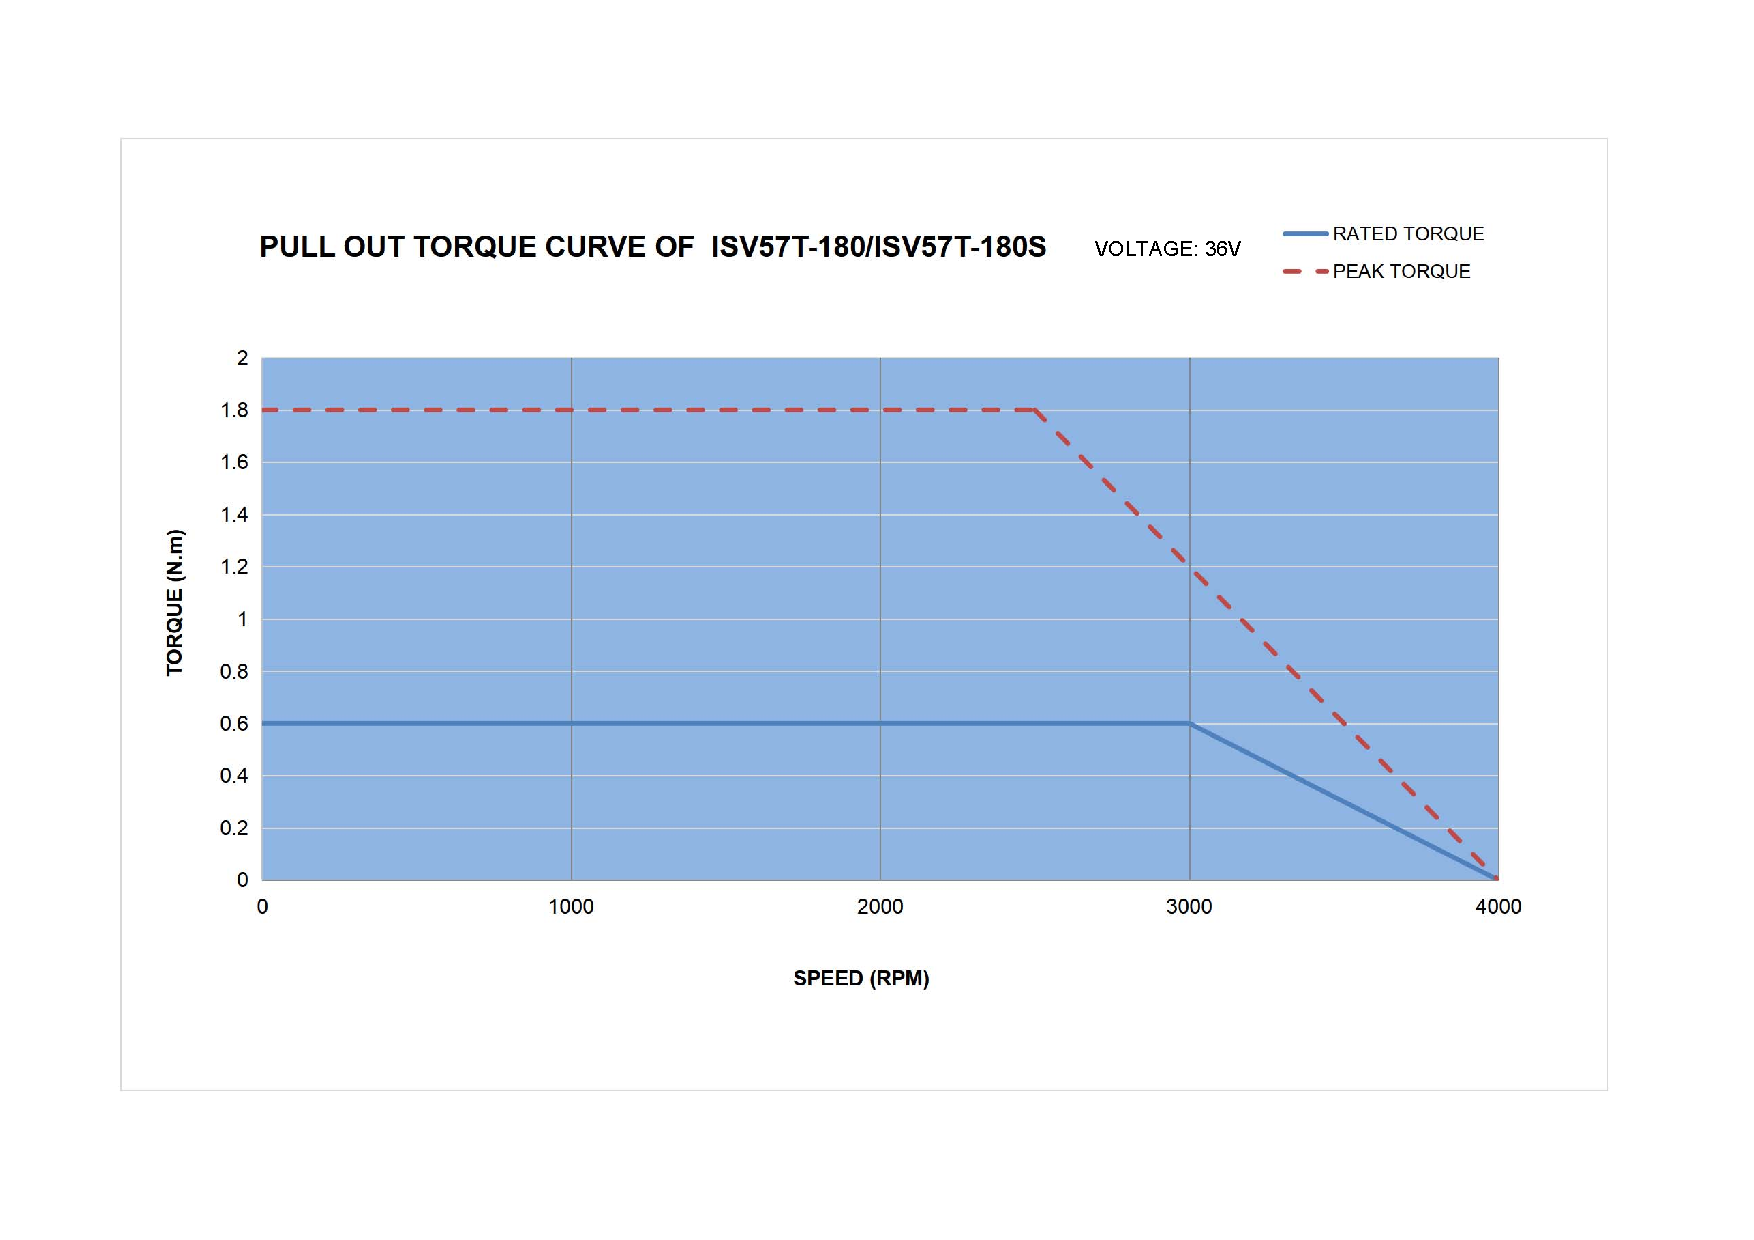
\includegraphics[width=0.85\textwidth]{ISV57T-180S_Torque_Speed_Curve.pdf}
    \caption{Torque--speed curve, StepperOnline iSV57T-180S.}
    \label{fig:full_scale_motor_torque_curve}
\end{figure}

\section{Scaled Test Actuator System}

\subsection{Assumed Test-System Parameters}

\begin{table}[h!]
\centering
\begin{tabularx}{\textwidth}{@{}l Y l@{}}
\toprule
\textbf{Parameter} & \textbf{Description} & \textbf{Value} \\
\midrule
$L_1$ & Beam length & $1.0\ \mathrm{m}$ \\
$L_2$ & Payload length along rail & $0.5\ \mathrm{m}$ \\
$m_1$ & Beam mass & $1.67\ \mathrm{kg}$ \\
$m_2$ & Payload mass & $5.0\ \mathrm{kg}$ \\
$r_{m_2}$ & Payload CM from pivot & $0.75\ \mathrm{m}$ \\
$r_f$ & Actuator attach from pivot & $0.5\ \mathrm{m}$ \\
$\Delta\theta$ & Angular travel & $10^\circ$ \\
$T$ & Motion time & $0.5\ \mathrm{s}$ \\
$L_s$ & Screw lead (selected hardware) & $0.00635\ \mathrm{m/rev}$ ($0.25\ \mathrm{in}$) \\
$\eta$ & Acme efficiency (assumed) & $0.60$ \\
\bottomrule
\end{tabularx}
\caption{Scaled test-system assumptions.}
\end{table}

\subsection{Required Actuator Performance}

\begin{table}[h!]
\centering
\begin{tabularx}{\textwidth}{@{}Y l@{}}
\toprule
\textbf{Calculated quantity} & \textbf{Result} \\
\midrule
Angular acceleration & $2.793\ \mathrm{rad/s^2}$ \\
Maximum actuator force & $109.4\ \mathrm{N}$ \\
Recommended force ($2\times$ SF) & $218.7\ \mathrm{N}$ \\
Linear travel ($r_f\sin\Delta\theta$) & $0.087\ \mathrm{m}$ \\
Average linear speed & $0.174\ \mathrm{m/s}$ \\
Motor torque at SF force & $0.368\ \mathrm{N\,m}$ \\
Screw speed (average / triangular peak) & $1641\ /\ 3282\ \mathrm{RPM}$ \\
\bottomrule
\end{tabularx}
\caption{Scaled sizing with outboard $r_{m_2}$ and selected lead.}
\end{table}

\subsection{Selected Test-System Components}

\begin{table}[h!]
\centering
\begin{tabularx}{\textwidth}{@{}l Y Y@{}}
\toprule
\textbf{Component} & \textbf{Selected part / relevant specification} & \textbf{Supplier link} \\
\midrule
Motor & StepperOnline iSV57T-090; $90\ \mathrm{W}$, $0.3\ \mathrm{N\,m}$ rated, $3000\ \mathrm{RPM}$ rated, $20$--$50\ \mathrm{VDC}$, $8\ \mathrm{mm}$ shaft. & \href{https://www.stepperonline.ca/nema-23-integrated-easy-servo-motor-90w-3000rpm-0-3nm-42-49oz-in-20-50vdc-brushless-dc-servo-motor-isv57t-090.html}{iSV57T-090} \\
\addlinespace
Lead screw & McMaster-Carr 99030A986; $3/8$ in--8 Stub Acme, two-start, $0.25$ in lead, $18$ in, 1018 steel. & \href{https://www.mcmaster.com/99030A986/}{99030A986} \\
\addlinespace
Lead nut & McMaster-Carr 1349K107; matching PET nut; dynamic thrust $350\ \mathrm{lbf}$. & \href{https://www.mcmaster.com/1349K107/}{1349K107} \\
\addlinespace
Shaft coupler & $5/16$ in to $5/16$ in set-screw coupler; temporary fix or weld for the test bed. & \href{https://abra-electronics.com/robotics-actobotics-servocity/motion-en/couplers/set-screw-shaft-couplers/625126-5-16-to-5-16-set-screw-shaft-coupler-actobotics-clone.html}{Abra 625126} \\
\bottomrule
\end{tabularx}
\caption{Selected scaled test-system components.}
\end{table}

\subsection{Test Motor Selection Rationale}

SF torque demand is $0.37\ \mathrm{N\,m}$ vs $0.3\ \mathrm{N\,m}$ rated
($0.8\ \mathrm{N\,m}$ peak). Rated torque is tight; peak torque covers the SF
case. Screw speeds sit inside the $4000\ \mathrm{RPM}$ max.

\begin{figure}[H]
    \centering
    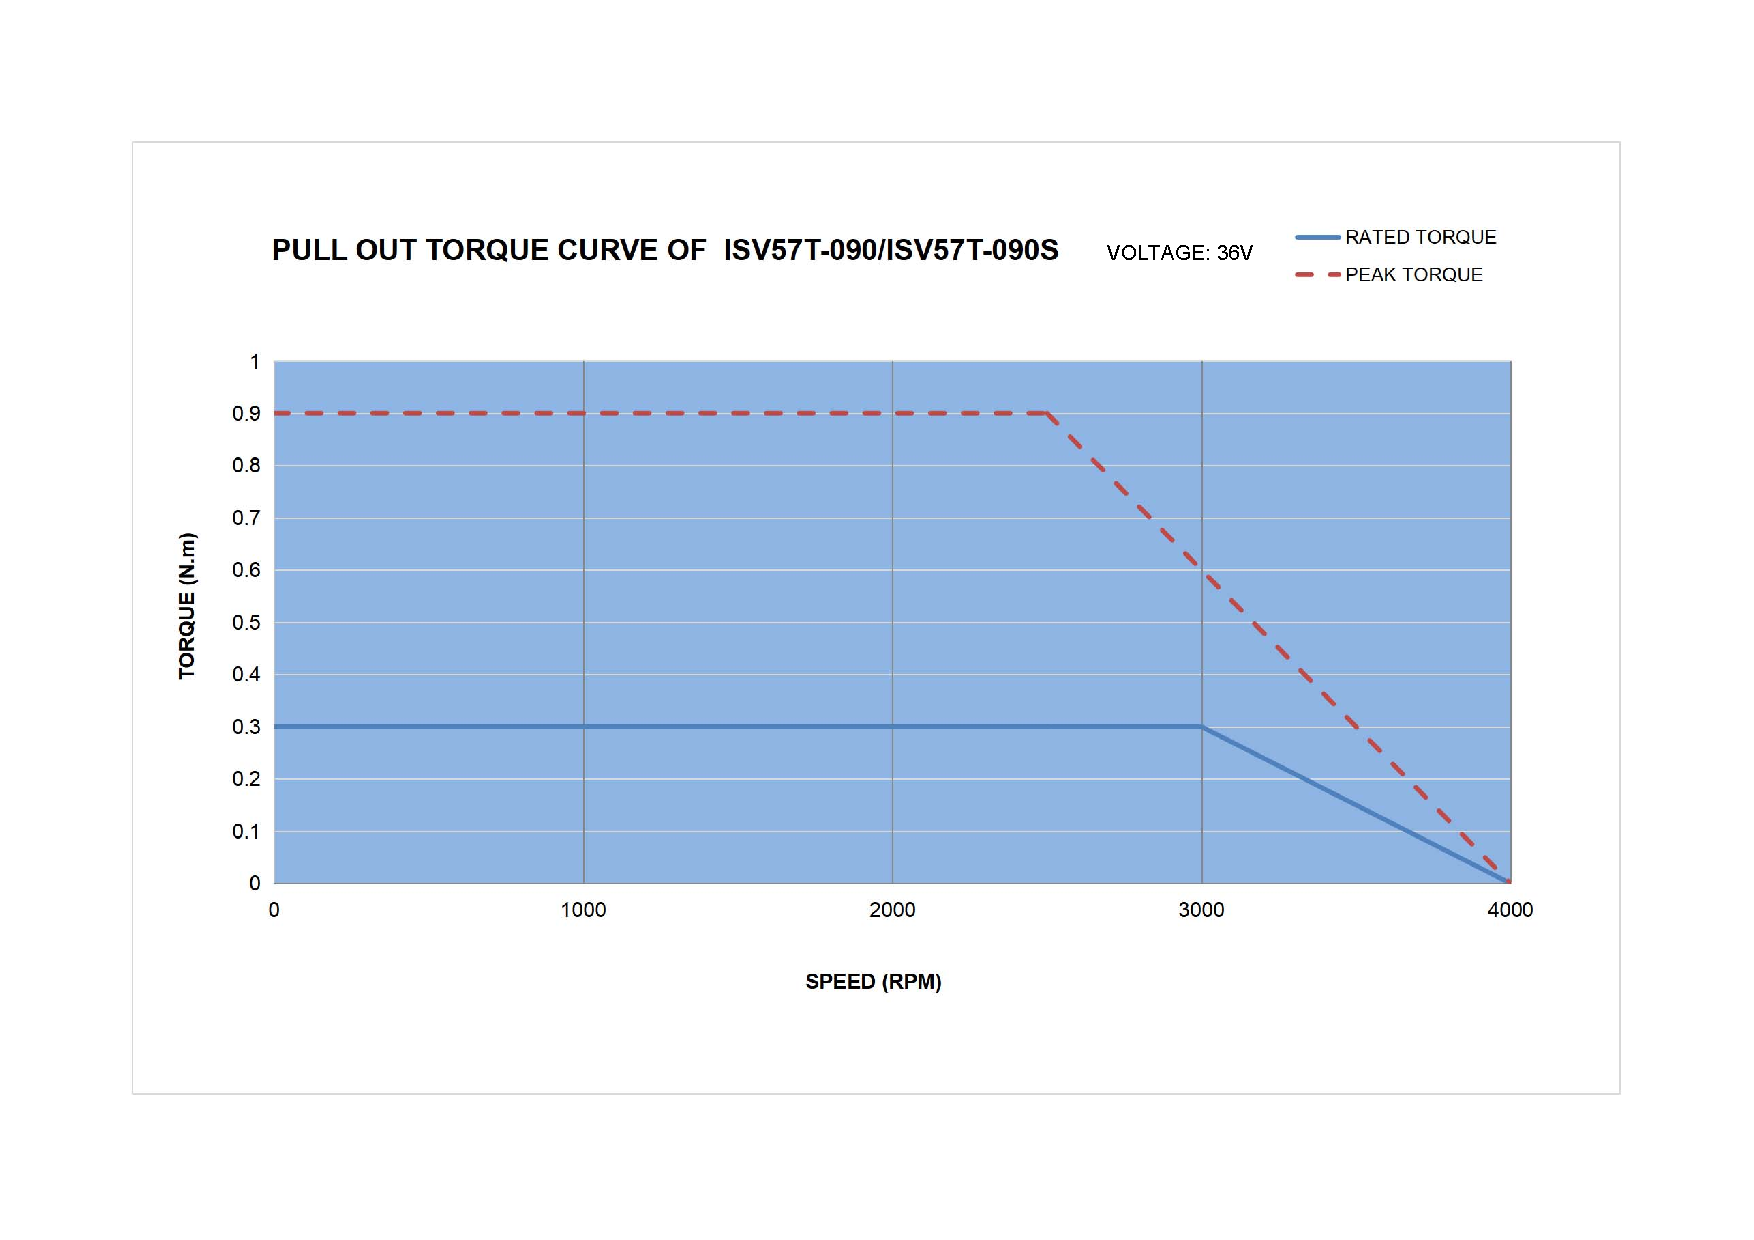
\includegraphics[width=0.85\textwidth]{nema-23-stepper-motor-specs.pdf}
    \caption{Torque--speed curve, StepperOnline iSV57T-090.}
    \label{fig:test_motor_torque_curve}
\end{figure}

\section{Selection Summary}

\begin{table}[h!]
\centering
\begin{tabularx}{\textwidth}{@{}l Y Y@{}}
\toprule
\textbf{Item} & \textbf{Full-scale} & \textbf{Scaled test} \\
\midrule
Motor & iSV57T-180S, $180\ \mathrm{W}$, $0.6\ \mathrm{N\,m}$ rated & iSV57T-090, $90\ \mathrm{W}$, $0.3\ \mathrm{N\,m}$ rated \\
Screw & 98980A973, $0.5$ in lead Acme & 99030A986, $0.25$ in lead Acme \\
Nut & 1349K101 & 1349K107 \\
Force (SF~$2$) & $169\ \mathrm{N}$ & $219\ \mathrm{N}$ \\
Torque (SF~$2$) & $0.57\ \mathrm{N\,m}$ & $0.37\ \mathrm{N\,m}$ \\
Screw speed (avg / peak) & $2871\ /\ 5743\ \mathrm{RPM}$ & $1641\ /\ 3282\ \mathrm{RPM}$ \\
Control / power & Arduino STEP/DIR; $\sim 36\ \mathrm{V}$ pack & same \\
\bottomrule
\end{tabularx}
\caption{Selected parts vs corrected sizing.}
\end{table}

\begin{thebibliography}{00}

\bibitem{stepperonline180}
STEPPERONLINE, ``NEMA 23 Integrated Easy Servo Motor 180W, iSV57T-180S.''
\url{https://www.stepperonline.ca/nema-23-integrated-easy-servo-motor-180w-3000rpm-0-6nm-84-98oz-in-20-50vdc-servo-motor-short-shaft-isv57t-180s.html}.
[Accessed: Nov. 12, 2026].

\bibitem{stepperonline090}
STEPPERONLINE, ``NEMA 23 Integrated Easy Servo Motor 90W, iSV57T-090.''
\url{https://www.stepperonline.ca/nema-23-integrated-easy-servo-motor-90w-3000rpm-0-3nm-42-49oz-in-20-50vdc-brushless-dc-servo-motor-isv57t-090.html}.
[Accessed: Nov. 12, 2026].

\bibitem{full_leadscrew}
McMaster-Carr, Part No.\ 98980A973. \url{https://www.mcmaster.com/98980A973/}.

\bibitem{full_leadnut}
McMaster-Carr, Part No.\ 1349K101. \url{https://www.mcmaster.com/1349K101/}.

\bibitem{full_coupler}
Abra Electronics, Part No.\ 625182.
\url{https://abra-electronics.com/robotics-actobotics-servocity/motion-en/couplers/set-screw-shaft-couplers/625182-1-4-to-8mm-set-screw-shaft-coupler-actobotics-clone.html}.

\bibitem{test_leadscrew}
McMaster-Carr, Part No.\ 99030A986. \url{https://www.mcmaster.com/99030A986/}.

\bibitem{test_leadnut}
McMaster-Carr, Part No.\ 1349K107. \url{https://www.mcmaster.com/1349K107/}.

\bibitem{test_coupler}
Abra Electronics, Part No.\ 625126.
\url{https://abra-electronics.com/robotics-actobotics-servocity/motion-en/couplers/set-screw-shaft-couplers/625126-5-16-to-5-16-set-screw-shaft-coupler-actobotics-clone.html}.

\end{thebibliography}

\end{document}
